\section{The PDF Trust Chain \note{1.5pp}}
\label{sec:trust-chain}

\subsection{Trust Chains in General}
The term \emph{Trust Chain} (or ``Chain of Trust'') is used in multiple contexts, e.g.,
\emph{digital certificates}: a sequence of certificates signing certificates,
starting with a root certificate;
\emph{supply chain}: a product is no more reliable or secure than its
outsourced components;
\emph{trusted boot}: unless the bootloader is correct and non-malicious,
there can be no possibility of the operating system being the same;
\emph{software stacks}: upper layers are dependent upon lower layers (such as
system libraries) and vulnerabilities at the lower layers affect all higher layers.

The common idea is having layers
that rely on lower layers for their validity
(or components that rely on sub-components, etc.),
and the key lesson being:
{\bf{if a single layer of the trust chain 
  is flawed or suborned, then every layer relying on it
  is no longer capable of being trusted.}}

\mtnote{I used 'layer' in this subsection, but hereafter I'll be using
  'stage' (not phase/component/etc) for our concrete instance in PDF.}

\subsection{The Trust Chain of a PDF Parser}

% In \cref{sec:pdf-challenges}, we elaborated on the challenges of PDF.
% Parsing data-formats has a long history and many solutions ...
% Parsing formal languages also has a long history and many solutions ...
% PDF has aspects of both: this makes PDF challenging.
% But PDF ``parsing'' is not merely a matter of harder [difference of degree]
% but intrinsically more complex [a difference of kind!]:

\begin{figure}[t]
  \centering
  \begin{lstlisting}
    +-----------------------------------------------------+
    | 1. Find & parse header and trailer                  |<-- File
    +-----------------------------------------------------+
                       | offsets + ...
                       v
    +-----------------------------------------------------+
    | 2. Find & parse incremental updates                 |<-- File
    +-----------------------------------------------------+
                       | list of raw XRef maps
                       v
    +-----------------------------------------------------+
    | 3. Combine incremental updates                      |<-- File
    +-----------------------------------------------------+
                       | one XRef map
                       v
    +-----------------------------------------------------+
    | 4. Transform XRef map to object map (DOM)           |
    |    1. Parse uncompressed objects                 <--+-- File
    |    2. Decode streams & preprocess object streams <--+-- File
    |    3. Resolve type 2 object references           <--+-- File
    +-----------------------------------------------------+
                       | Object map (DOM)
                       v
    +-----------------------------------------------------+
    | 5. Validate candidate DOM                           |
    +-----------------------------------------------------+
                       | Object map (DOM)                                    
                       v
    +-----------------------------------------------------+
    | 6. Render DOM                                       |
    +-----------------------------------------------------+
                       | 
                       v
  \end{lstlisting}
  % 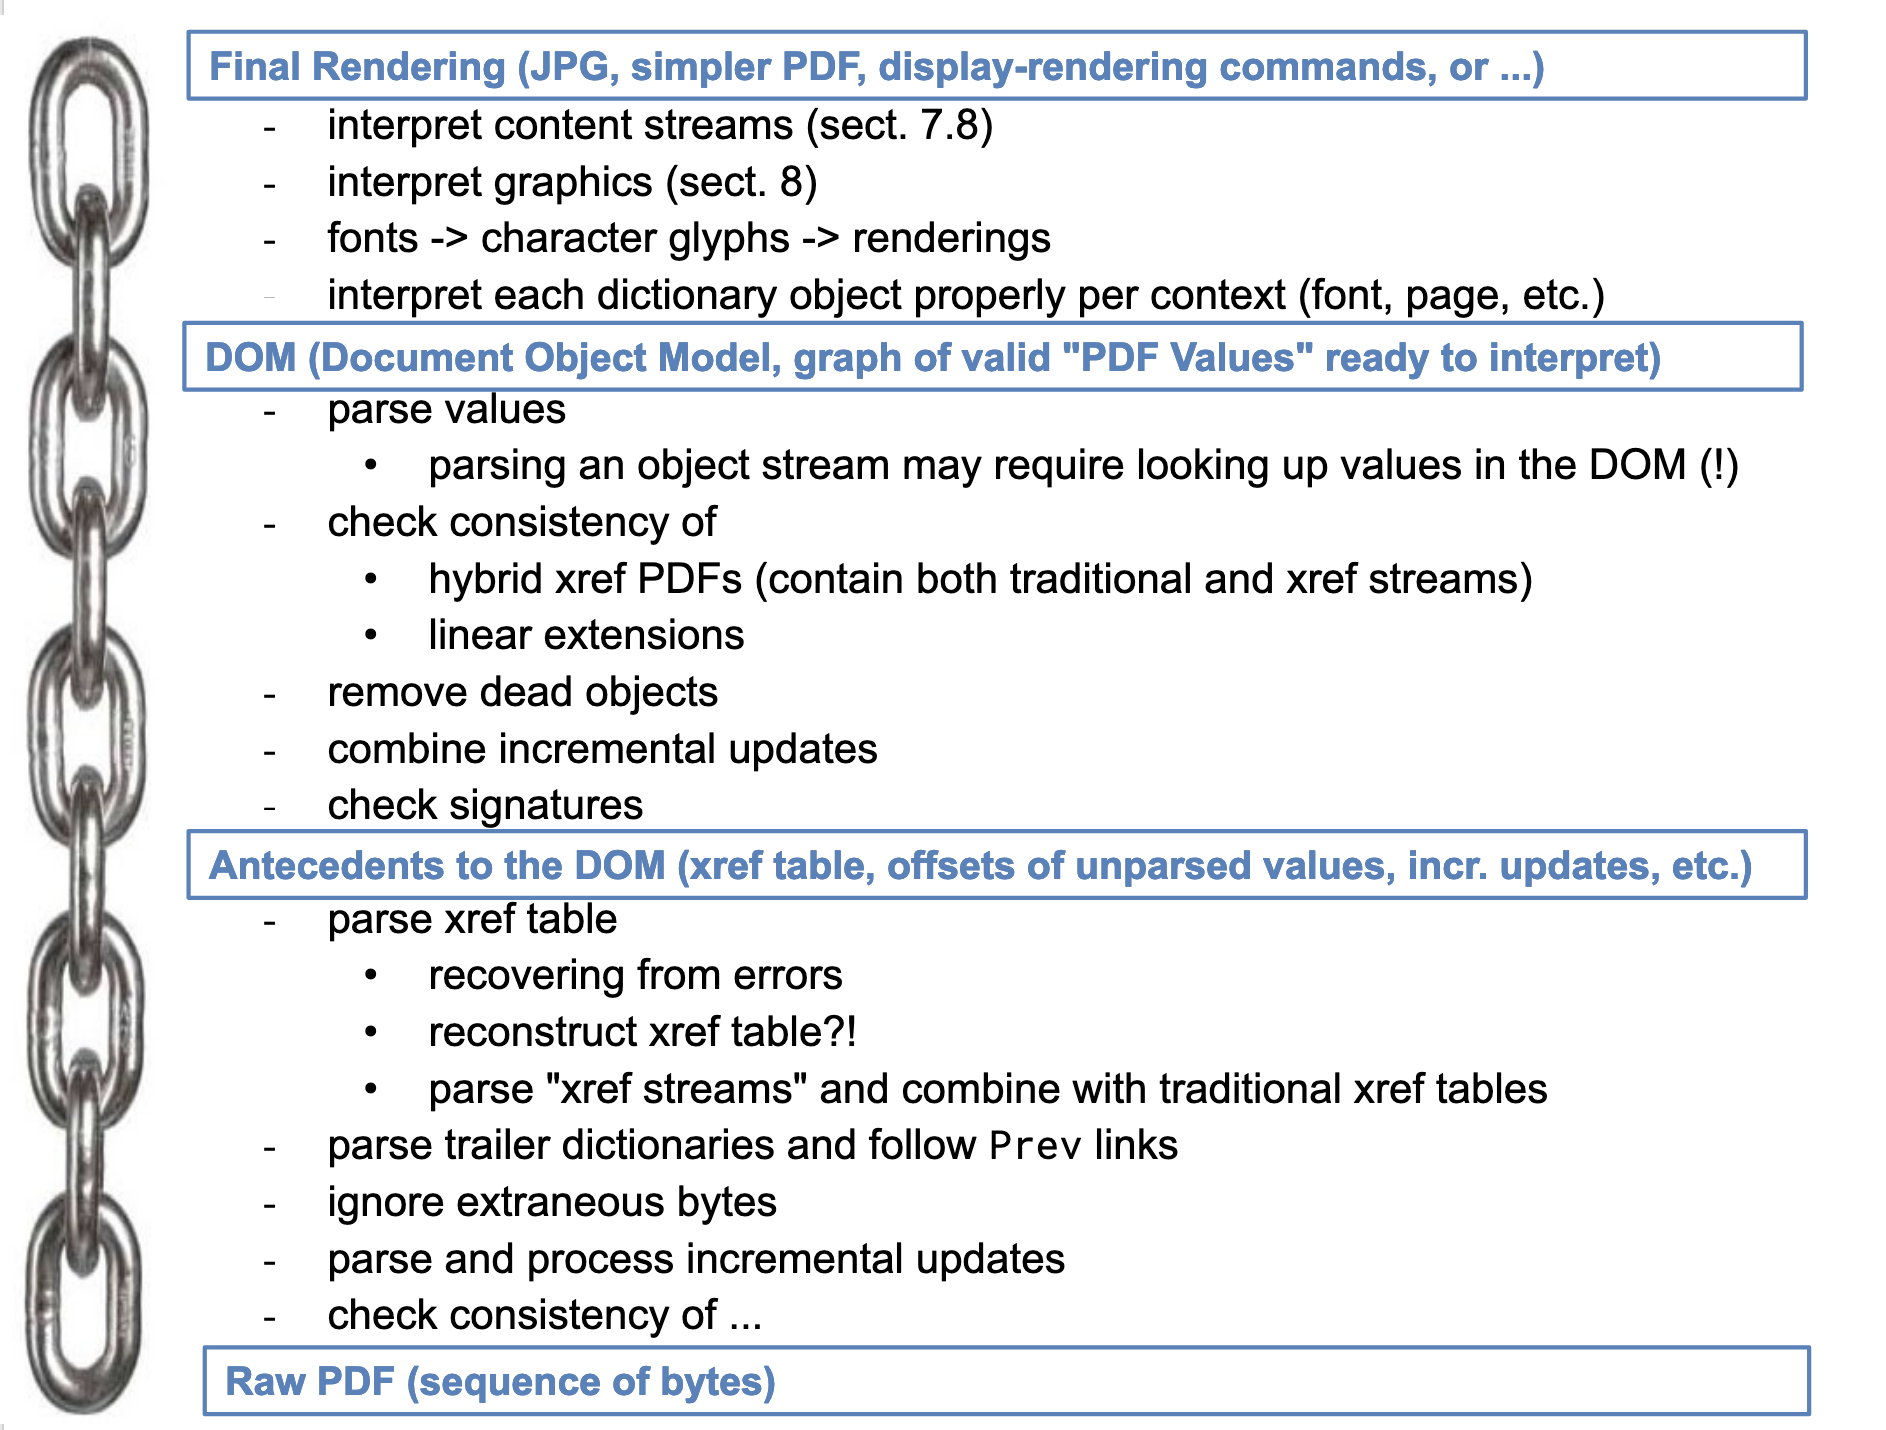
\includegraphics[width=0.8\linewidth]{figures/trustchain-diagram.png}
  \caption{Stages of PDF Parsing (the Trust Chain)}
  \mttodo{un-ascii-ify diagram}
  \label{fig:pdf-trust-chain}
\end{figure}

We have touched upon the complexities of parsing
PDF, but to appreciate these, one has to understand the
dependencies and interactions between the features.
In \cref{fig:pdf-trust-chain} we show the main stages diagrammatically.
To briefly sketch what's going on in each stage:
\begin{itemize}
\item Stage 1: Find and parse both the PDF header and the PDF trailer to locate
  the document trailer dictionary and the start of the last incremental update or
  the cross reference table of the original document in the case of no updates.
\item Stage 2: Find and parse each cross reference table or incremental update. 
  Note that this stage uses context from Stage 1 (such as the file offset and trailer
  information) in order to know  \emph{where} to start processing.
\item Stage 3: This stage does no further reading of the file, but computes the
   a XRef map of the final PDF by accounting for each set of edits performed by each incremental update.
   Incremental updates can add new objects, mark as free previous objects, re-instate previously 
   freed objects, and change context information in the trailer dictionary that 
   forms part of each incremental update.
\item Stage 4: Transform XRef map to object map. This stage is complex and
  requires three sub-stages, each of which does further file input and parsing.
  Further details are in \cref{sec:specifying}.
  If all goes well, we have a syntactically correct DOM.
\item Stage 5: Validate candidate DOM.  This stage takes the candidate DOM and
  semantically verifies that it represents a sensible Document Tree per the PDF Standard.
  E.g., each object in the DOM is well formed with required data types and values, 
  no unexpected recursion, etc.
\item Stage 6: Render DOM.  Here we render the validated DOM, or parts thereof,
  to the output format of choice.
\end{itemize}

Any error (malicious or otherwise) in an earlier stage will affect the output of stages that follow.
But note stages 2, 3, 4.1, 4.2, and 4.3 all depend on inputs from the previous stage to determine 
where and how to parse segments of the PDF input file.
Errors that percolate into these stages can
cause all forms of havoc (parsing wrong data, etc.).
%
The attentive reader will note that we have another instance of a \emph{Trust
Chain}.  The subsequent stages of the parsing process are \emph{completely
dependent} upon the earlier stages to properly parse and interpret the PDF
file.

An implementation \emph{might} merge stages 2, 3, 4.1, 4.2, 4.3 into
a single stage and give a \emph{semblance} of simplicity.
%
Our argument in what follows---particularly in
\cref{sec:single-pass-problems}---is
that such an implementation will be overly
complex and be a design for which it is highly intractable
to determine that it implements the standard
and to determine that it terminates for all input files.

We think it is important to understand PDF parsing in terms of this
\emph{Trust Chain} because
%
(1) it highlights the presence of the many ``dependent'' stages
in PDF processing;
%
(2) it highlights the importance of ensuring the pre-DOM parsing, data integrity relationships and
computation (the base of our Trust Chain) is correct and secure;
%
(3) it reminds us that the integrity of the DOM cannot be verified
independently of verifying all the earlier stages; and
%
(4) it illustrates that PDF parsing, although uniquely complex, is an instance of
a general concept.

Although \emph{Validate candidate DOM} (stage 5) might be considered tedious, the necessary checks are 
reasonably well defined by the bulk of the PDF Standard. Validation involves ensuring that each 
individual PDF object has all the required keys and appropriate values in the context of its reference in the DOM.
For example, a PDF object that is a thumbnail for a PDF needs to be an Image XObject and have a 
minimum set of required key names and their values each within predefined limits (e.g. both
\lstcd{Height} and \lstcd{Width} are required keys and must be non-negative integers). If the 
thumbnail reference in the candidate DOM is to a font dictionary or some other kind of
\emph{syntactically} valid PDF object then this is \emph{semantically} incorrect. Recent work
\cite{arlingtonPdfModel} created the first specification-derived comprehensive
machine-readable model of every object, their attributes and relationships in the PDF DOM. The use
of such a model for code generation, validation or test case generation can reduce the tediousness.


The \emph{Render DOM} stage also has many complications of its own, whether this be rendering a PDF
page to pixels for display or print, or extracting text contract, however for this paper we will
focus on stages 1-4.

We refer to stages 1 to 4 as pre-DOM parsing/computation; if anything
goes wrong pre-DOM---and lots can go wrong---there's hell to pay.
\todo{do we dare?!}

\todo{BH: I urge against: it's not so much that the tone is too
  risque, but (related) that it's not suitably precise.}
